We performed resolution tests for models with [Fe/H] $\in \{-1.2, -0.4, 0.4\}$ and $M \in \{0.9, 1.3, 1.7\}$ using the Brown thermohaline mixing prescription.
We studied a grid of \texttt{mesh\_delta\_coeff} and \texttt{time\_delta\_coeff} values which span from 0.1 to 1.0 over five log-space steps.
This means that we evolved simulations with both spatial and temporal resolutions ranging from $1\times$ to $10\times$ the default resolutions.
For each simulation, we evolve the 1D stellar model as described in Sec.~\ref{sec:mesa_experiment}, then decrease (or increase) the spatial and temporal resolution on the red giant branch once $\log g \leq 3$.
We measure the inverse density ratio $r$ in each of these models, and in Fig.~\ref{Fig:resolution_test} we plot the absolute value of the percentage difference between that $r$ value and the reference $r_{\rm ref}$ value reported for that case in Fig.~\ref{fig:mesa_r_spread}.
We calculate the percentage difference to be $100(1 - r/r_{\rm{ref}})$.

We find that small values of the mesh coefficient (high spatial resolution) combined with large values of the time coefficient (large timesteps) result in large errors.
This occurs because the front of the thermohaline zone, and sometimes the full thermohaline zone, becomes numerically unstable, and large oscillations in $R_0$ lead to large errors in the $r$ calculation.
Furthermore, we find that when the thermohaline front is not properly numerically resolved, it does not propagate upwards in mass coordinate and so does not connect with the convective shell.
This likely has important implications for the evolution (or lack thereof) of surface abundances in these models.


\begin{figure*}[!tb]
\begin{center}
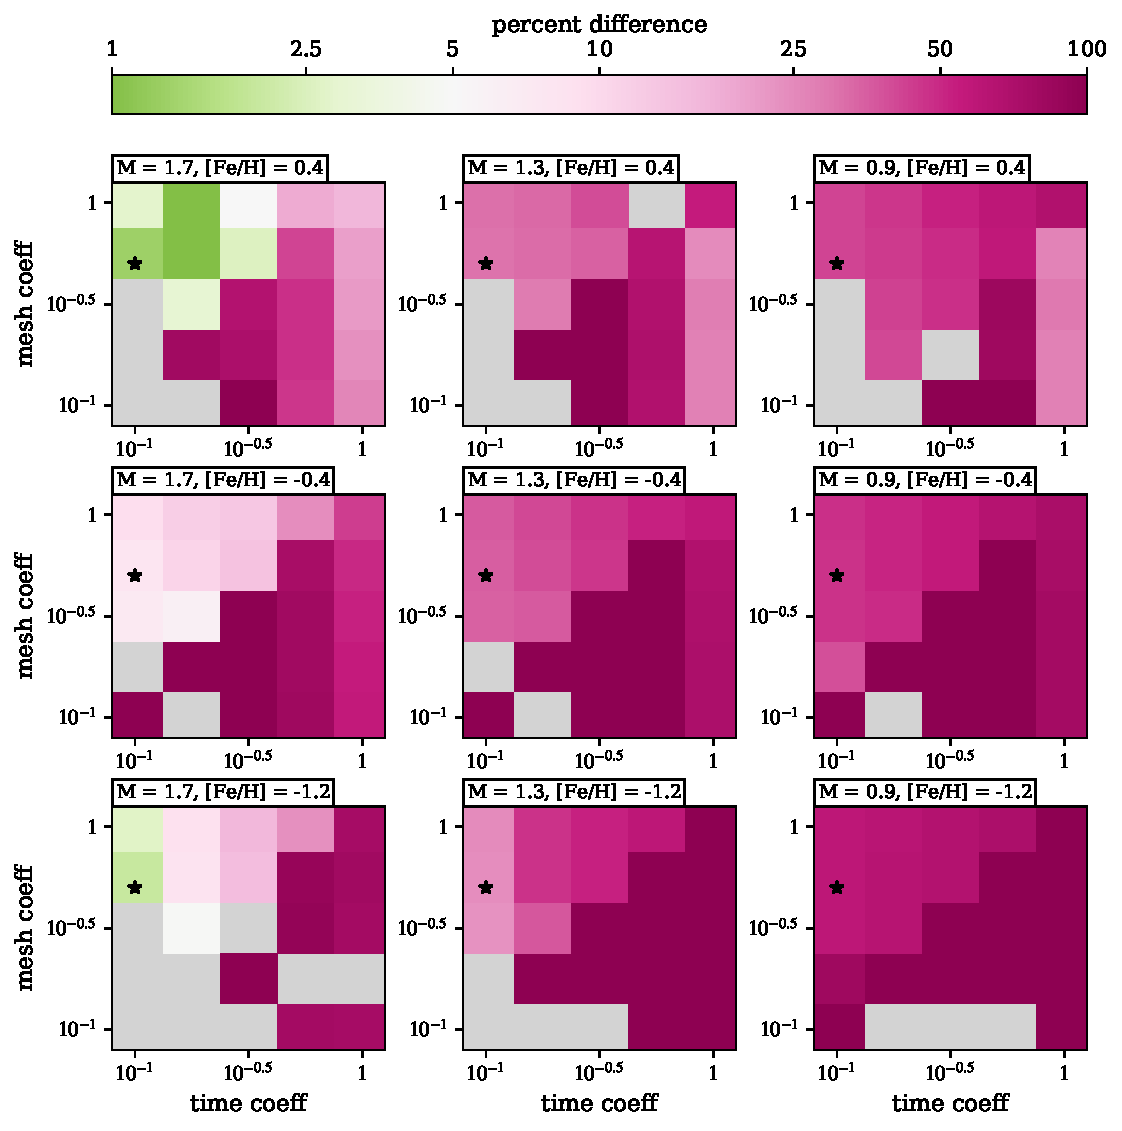
\includegraphics[width=\textwidth]{resolution_test.pdf}
\caption{
    We plot a 3x3 grid of colormaps corresponding to a grid of mass $M \in [0.9, 1.3, 1.7]$ and [Fe/H]$ \in [-1.2, -0.4, 0.4]$.
    At each mass and [Fe/H], we simulate a 5x5 grid of MESA models with varying spatial and temporal resolution.
    We plot in color the percent difference between the measured value of the reduced density ratio $r$ and its reference value reported in Fig.~\ref{fig:mesa_r_spread}.
    The resolution of the grids of simulations presented in Fig.~\ref{fig:mesa_r_spread} are marked by black stars.
    Cases with $r$ measurements within 5\% of the reference values are colored in green, while points with larger differences are colored pink.
    Grey pixels are simulations for which either there was a supercomputer error or the algorithm failed to identify a thermohaline zone.
    }
\label{Fig:resolution_test}
\end{center}
\end{figure*}